%-----------------------------------------------
%  Engineer's & Master's Thesis Template
%  Copyleft by Artur M. Brodzki & Piotr Woźniak
%  Warsaw University of Technology, 2019-2022
%-----------------------------------------------

\documentclass[
    bindingoffset=5mm,  % Binding offset
    footnoteindent=3mm, % Footnote indent
    hyphenation=true    % Hyphenation turn on/off
]{src/wut-thesis}

\graphicspath{{tex/img/}} % Katalog z obrazkami.
\addbibresource{bibliografia.bib} % Plik .bib z bibliografią

%-------------------------------------------------------------
% Wybór wydziału:
%  \facultyeiti: Wydział Elektroniki i Technik Informacyjnych
%  \facultymeil: Wydział Mechaniczny Energetyki i Lotnictwa
% --
% Rodzaj pracy: \EngineerThesis, \MasterThesis
% --
% Wybór języka: \langpol, \langeng
%-------------------------------------------------------------
\facultyeiti    % Wydział Elektroniki i Technik Informacyjnych
\MasterThesis % Praca inżynierska
\langeng % Praca w języku polskim

\begin{document}

%------------------
% Strona tytułowa
%------------------
\instytut{Computer Science}
\kierunek{Computer Science}
\specjalnosc{Computer Systems and Networks}
\title{Developing a New Pruning Method for CVFDT: A Study on\\Lazy Pruning in Data Stream Mining}
\engtitle{Developing a New Pruning Method for CVFDT: A Study on\\Lazy Pruning in Data Stream Mining}
\poltitle{Opracowanie nowej metody przycinania dla CVFDT:\\badanie leniwego przycinania w eksploracji strumieni danych}
\author{Nityanand Waingankar}
\album{336962}
\promotor{Izabela Zoltowska}
\date{\the\year}
\maketitle

%-------------------------------------
% Streszczenie po polsku dla \langpol
% English abstract if \langeng is set
%-------------------------------------
\cleardoublepage % Zaczynamy od nieparzystej strony
\abstract
This thesis evaluates Lazy Very Fast Decision Trees (Lazy VFDT) against Dynamic Weighted Majority for concept-drifting data streams. Lazy VFDT combines Hoeffding-tree growth with lazy pruning at prediction time, aiming to match ensemble accuracy with far lower training and inference cost. Experiments on synthetic drift, Electricity, Gas Sensor, and Airlines streams show that Lazy VFDT often matches or exceeds the baseline on gradual drift with orders-of-magnitude efficiency gains, and remains competitive on harder multi-class streams with modest tuning and scaling.
\keywords data streams, concept drift, lazy pruning, Hoeffding tree, CVFDT, VFDT, dynamic weighted majority


%----------------------------------------
% Streszczenie po angielsku dla \langpol
% Polish abstract if \langeng is set
%----------------------------------------
\clearpage
\secondabstract
Niniejsza praca ocenia Lazy Very Fast Decision Trees (Lazy VFDT) w porównaniu z Dynamic Weighted Majority dla strumieni danych z dryfem koncepcji. Lazy VFDT łączy rozwój drzewa Hoeffding z leniwym przycinaniem w czasie predykcji, aby osiągnąć dokładność zbliżoną do zespołów przy znacznie niższych kosztach uczenia i wnioskowania. Eksperymenty na syntetycznych dryfach, Electricity, Gas Sensor i Airlines pokazują, że Lazy VFDT często dorównuje lub przewyższa bazę na łagodnym dryfie, oferując rzędy wielkości lepszą efektywność, i pozostaje konkurencyjny na trudniejszych wieloklasowych strumieniach przy umiarkowanym strojeniu i skalowaniu.
\secondkeywords strumienie danych, dryf koncepcji, leniwe przycinanie, drzewo Hoeffding, CVFDT, VFDT, dynamic weighted majority

\pagestyle{plain}

%--------------
% Spis treści
%--------------
\cleardoublepage % Zaczynamy od nieparzystej strony
\tableofcontents

%------------
% Rozdziały
%------------
\cleardoublepage % Zaczynamy od nieparzystej strony
\pagestyle{headings}

\cleardoublepage
\chapter{Introduction}
\label{chap:introduction}

\section{Motivation}
Continuous data streams are now the norm for cyber-physical systems, smart infrastructure, and interactive services.  Unlike stationary datasets, streams evolve as user behaviour, physical environments, and sensing hardware drift over time.  Concept drift invalidates static models \cite{gama2014survey}, yet industry systems still need real-time predictions delivered at millisecond latency.  Ensemble-based stream learners, such as Dynamic Weighted Majority (DWM) \cite{kolter2007dwm}, provide strong accuracy but at the cost of expensive updates and high prediction latency.  For resource-constrained deployments and safety-critical feedback loops, the computational overhead of retraining large ensembles is prohibitive.  This motivates the study of lightweight streaming models that adapt fast, remain interpretable, and have predictable latency profiles.

\section{Problem Statement and Objectives}
This thesis investigates Lazy Very Fast Decision Trees (Lazy VFDT) as an alternative to ensemble methods for concept-drifting streams.  Lazy VFDT combines incremental Hoeffding-tree style growth \cite{domingos2000vfdt} with a ``lazy'' pruning step executed during prediction.  The central research problem is whether this design can match the accuracy of established baselines while dramatically lowering training and inference costs.  The concrete objectives are:
\begin{itemize}
    \item Design and stabilise an implementation of Lazy VFDT that supports single-instance updates, lazy pruning, and reproducible experimentation.
    \item Establish a fair baseline with DWM using identical feature sets and data streams.
    \item Evaluate both approaches on synthetic and real-world drift benchmarks, measuring accuracy, training time, average and p95 prediction latency, and model size.
    \item Analyse how dataset characteristics (gradual vs. sudden drift, binary vs. multi-class labels) and preprocessing choices (feature scaling, batch-aware normalisation) influence model behaviour.
\end{itemize}

\section{Contributions}
The thesis delivers the following contributions:
\begin{enumerate}
    \item A reproducible Python framework that streams instances to Lazy VFDT and DWM under identical conditions, logs metrics per seed, and automates result aggregation.
    \item Dataset loaders and preprocessing pipelines for the canonical Electricity dataset, the Gas Sensor Array Drift benchmark, Airlines flight-delay data, and rotating hyperplane generators, including tooling for per-batch scaling and libsvm-to-CSV conversion.
    \item An empirical study across these benchmarks demonstrating where Lazy VFDT matches or exceeds DWM accuracy while reducing training time by one to two orders of magnitude and lowering prediction latency.
    \item Guidance on dataset-specific presets (e.g., per-batch scaling for sensor drift, deeper trees for multi-class streams) that practitioners can reuse when deploying Lazy VFDT.
\end{enumerate}

\section{Thesis Structure}
The remainder of the document follows the structure below:
\begin{itemize}
    \item Chapter~\ref{chap:related-work} summarises related work on concept drift, Hoeffding trees, and ensemble stream learners.
    \item Chapter~\ref{chap:methodology} details the Lazy VFDT architecture, the DWM baseline, implementation specifics, and dataset preprocessing pipelines.
    \item Chapter~\ref{chap:setup} describes the experimental protocol, metrics, hardware, and tooling used to ensure reproducibility.
    \item Chapter~\ref{chap:results} presents quantitative results with aggregated tables and plots, comparing accuracy, training time, latency, and model size across datasets.
    \item Chapter~\ref{chap:discussion} discusses the implications of these findings, highlighting strengths, limitations, and practical recommendations.
    \item Chapter~\ref{chap:conclusion} concludes the thesis and outlines directions for future work on adaptive parameter tuning and additional baselines.
\end{itemize}
              % Wygodnie jest trzymać każdy rozdział w osobnym pliku.
\cleardoublepage
\chapter{Related Work}
\label{chap:related-work}

This chapter reviews the foundations of streaming classification with concept drift and situates Lazy VFDT within existing literature on Hoeffding trees, ensemble learners, and dataset benchmarks used by the streaming community.

\section{Concept Drift in Data Streams}
Streaming models must operate under a constrained memory budget while reacting to non-stationary distributions \cite{gama2014survey}.  Drift is typically categorised as:
\begin{itemize}
    \item \textbf{Gradual drift}---the decision boundary moves slowly over time (e.g., seasonal electricity demand).  Prequential evaluation and sliding windows are common countermeasures.
    \item \textbf{Sudden drift}---an abrupt regime change (e.g., sensor recalibration).  Detection-and-reset mechanisms or ensembles with change detectors are often used.
    \item \textbf{Recurring drift}---concepts reappear after periods of absence, requiring learners to retain historical knowledge without memorising all data.
\end{itemize}
Handling drift efficiently requires streaming learners to support instance-wise updates, bounded latency, and selective forgetting.  This motivates algorithms such as Very Fast Decision Trees (VFDT) and their derivatives.

\section{Decision Trees for Streams}
Hoeffding trees approximate batch decision trees by exploiting the Hoeffding bound to make split decisions using a small sample \cite{domingos2000vfdt}.  Notable enhancements include:
\begin{itemize}
    \item \textbf{VFDTc/VFDT-nc}: incorporate continuous attributes or numeric counters for better split confidence.
    \item \textbf{CVFDT}: maintain alternate subtrees to adapt to drift without rebuilding the entire model.
    \item \textbf{Probabilistic/VFDT-FR}: integrate feature re-weighting or naive Bayes leaves to improve accuracy under limited depth.
\end{itemize}
Lazy VFDT extends this family by postponing pruning until prediction time.  Internal nodes retain majority-class statistics and evaluate pruning criteria only when queried.  This ``lazy pruning'' reduces update cost (no eager restructuring) while enabling rapid recovery when drift renders a branch obsolete.

\section{Ensemble Approaches}
Ensemble learners dominate many concept-drift benchmarks thanks to their diversity and adaptive weighting.  Representative methods include:
\begin{itemize}
    \item \textbf{Dynamic Weighted Majority (DWM)} \cite{kolter2007dwm}: maintains a pool of experts with exponentially decayed weights, removing poorly performing experts and adding new ones upon errors.
    \item \textbf{Adaptive Random Forests} \cite{bifet2009arf}: combine multiple Hoeffding trees with online bagging and concept-drift detectors to selectively replace trees.
    \item \textbf{Leveraging Bagging}: increases classifier diversity via re-sampling tricks (e.g., Poisson sampling with ADWIN drift detectors).
\end{itemize}
While ensembles deliver strong accuracy, they incur significant training-time overhead and higher inference latency because each instance must traverse many models.  The contrast between such ensembles and Lazy VFDT is central to this thesis: we quantify the efficiency gap and identify when accuracy remains comparable.

\section{Benchmark Datasets}
Concept-drift research frequently relies on a small set of synthetic and real streams, each stressing different learner properties:
\begin{itemize}
    \item \textbf{Rotating Hyperplane}: synthetic gradual or sudden drift controlled via drift rate and noise; widely used to test theoretical behaviour.
    \item \textbf{Electricity (ELEC2)}: reflects market demand changes; binary labels, recurring daily patterns, and moderate noise \cite{harries1999electricity}.
    \item \textbf{Gas Sensor Array Drift}: multi-class sensor data with strong calibration drift, requiring normalisation per batch or sensor \cite{vergara2012gas}.
    \item \textbf{Airlines Flight Delay}: long-range stream with heterogeneous categorical attributes, highlighting the impact of feature encoding and latency constraints.
\end{itemize}
This thesis utilises the same dataset families to demonstrate Lazy VFDT under gradual, sudden, multi-class, and noisy drift scenarios.

\section{Summary}
Prior work establishes a trade-off between accuracy and efficiency: ensembles such as DWM achieve robustness at the cost of computational complexity, whereas single-tree approaches adapt quickly but may underperform without tuning.  Lazy VFDT sits between these extremes by combining Hoeffding-tree updates with lazy pruning.  The following chapters detail our methodology, implementation, and empirical evaluation designed to rigorously test this balance.
       % Umożliwia to również łatwą migrację do nowej wersji szablonu:
\cleardoublepage
\chapter{Methodology}
\label{chap:methodology}

This chapter describes the design of the Lazy VFDT learner, the Dynamic Weighted Majority (DWM) baseline, the implementation choices made for this thesis, and the preprocessing pipelines used for each dataset.

\section{Lazy Very Fast Decision Tree}
Lazy VFDT inherits the incremental splitting strategy of Hoeffding trees while deferring pruning decisions until prediction time \cite{domingos2000vfdt}.  Each node stores:
\begin{itemize}
    \item split statistics (class counts per attribute) to evaluate splitting using Hoeffding bounds,
    \item the majority label routed through the node, used for both prediction and lazy pruning,
    \item pruning statistics tracking how many samples and misclassifications have passed through since the last pruning test.
\end{itemize}

\subsection{Update Procedure}
For every incoming instance, the algorithm:
\begin{enumerate}
    \item Traverses existing splits to reach a leaf, initialising the root on the first instance.
    \item Updates class counts at each visited node and refreshes the majority label.
    \item Every \texttt{grace\_period} instances, evaluates whether the leaf should split by computing information gain for a random subset of attributes, guided by the Hoeffding bound.
    \item If the best attribute exceeds the Hoeffding threshold, the node splits and initialises children with the current majority label.
\end{enumerate}
This approach guarantees logarithmic update time with respect to the number of nodes and permits bounded memory growth.

\subsection{Lazy Pruning During Prediction}
Traditional Hoeffding trees prune eagerly or rely on change detectors.  Lazy VFDT instead evaluates pruning only when the node is visited during prediction.  Given a test instance (optionally with its true label, as in prequential evaluation), the algorithm:
\begin{enumerate}
    \item Walks down the tree following split tests; if a node lacks children, it predicts using the stored majority label.
    \item Updates pruning statistics (sample count and misclassification count) for each node on the path.
    \item When the number of samples at a node exceeds a pruning grace period, compares the empirical misclassification rate with a confidence bound derived from the Hoeffding inequality.
    \item If the misclassification rate is below the bound, collapses the subtree into a leaf by discarding children and setting the node's prediction to its majority label.
\end{enumerate}
This ``lazy pruning'' avoids constant restructuring during updates, reducing training cost, while still reacting to drift when stale branches become unreliable.

\section{Dynamic Weighted Majority Baseline}
DWM maintains an ensemble of experts (decision trees) with weights adjusted according to performance \cite{kolter2007dwm}.  The implementation used here follows the canonical algorithm:
\begin{itemize}
    \item New experts are initialised with dummy data and added when the ensemble misclassifies.
    \item Weights are decayed by a factor \( \beta \) for experts that err on a given instance; experts with weights below \(\theta\) are removed.
    \item A sliding window buffers the most recent \(w\) instances to retrain experts periodically, providing adaptation to drift.
\end{itemize}
Predictions are obtained via weighted voting over all current experts.  While accurate, DWM's training time scales with the number of experts and window size, making it a computationally heavy baseline.

\section{Implementation Details}
Both models are implemented in Python (NumPy, scikit-learn) with a streaming driver (\texttt{compare\_lazy\_vs\_dwm.py}) that:
\begin{itemize}
    \item Streams instances from synthetic generators or preprocessed CSVs, preserving chronological order for real datasets.
    \item Supports multi-seed evaluation, logging accuracy, training time, per-instance latency, and model size to \texttt{results.csv}.
    \item Provides dataset-specific presets via command-line flags (e.g., \texttt{--preset gas}, \texttt{--scale-per-batch}).
\end{itemize}
Auxiliary tools include \texttt{tools/prepare\_gas\_sensor\_csv.py} for converting libsvm batches to a single CSV, \texttt{tools/summarize\_results.py} for aggregating metrics, and \texttt{tools/plot\_results.py} for generating figures.

\section{Dataset Preprocessing}
\subsection{Synthetic Rotating Hyperplane}
Gradual and sudden drift are simulated using a rotating hyperplane generator with tunable drift rate and noise.  Datasets are split into 70\% training (for streaming updates) and 30\% testing (for latency measurement).

\subsection{Electricity}
The ELEC2 dataset is converted from ARFF to CSV, with byte-prefixes removed from categorical attributes.  Chronological order is preserved; \texttt{date} and \texttt{day} fields are dropped, and the UP/DOWN label is mapped to \{0,1\}.  No additional scaling is applied.

\subsection{Gas Sensor Array Drift}
Raw batch files (libsvm format) are merged via \texttt{tools/prepare\_gas\_sensor\_csv.py}, producing a CSV with 128 features, batch identifiers, and categorical labels \cite{vergara2012gas}.  To combat sensor calibration drift, features are standardised per batch: a scaler is fit on the training portion of each batch and applied to both train and test subsets belonging to the same batch.

\subsection{Airlines}
Categorical fields (airline, airport, day-of-week) are one-hot encoded; numerical features are standardised globally.  Chronological order is maintained with a 70/30 split.  Given the dataset's scale and heterogeneity, deeper Lazy VFDT settings (\texttt{max\_depth=10}, \texttt{grace\_period=20}) and a larger DWM window are used to stabilise accuracy.

\section{Summary}
This methodology provides a controlled environment for comparing Lazy VFDT against DWM across diverse drift scenarios. The next chapter details the experimental protocol, metrics, evaluation flow, and tooling that ensures replicable results.        % zazwyczaj wystarczy podmienić plik src/wut-thesis.cls
\cleardoublepage
\chapter{Experimental Setup}
\label{chap:setup}

\section{Metrics}
We evaluate accuracy (percentage of correct predictions on the hold-out stream), total training time in seconds, per-instance prediction latency (mean and 95th percentile in milliseconds), and model size (node count for Lazy VFDT, number of experts for DWM). All metrics are recorded per seed and aggregated with mean and standard deviation using the tooling described in Section~\ref{chap:methodology}.

\section{Protocol}
Each dataset is streamed in chronological order (70\% train, 30\% test). For synthetic streams, we generate $10{,}000$ samples with specified drift rates/noise. For real datasets, we convert to CSV, preserve order, and split without shuffling. Each condition is repeated for seeds $\{13, 29, 47, 83, 101\}$; for synthetic data the seed controls random generation, while for real data it seeds model initialisation. Per-instance latency is measured using Python's \texttt{time.perf\_counter()} around the prediction call.

\section{Hardware and Software}
Experiments were run on a Windows 11 workstation using the \texttt{dtree} conda environment (Python 3.11, NumPy 2.1, scikit-learn 1.5, seaborn for plotting). Commands were executed via \texttt{conda run -n dtree python ...} to ensure reproducibility. Python scripts (\texttt{compare\_lazy\_vs\_dwm.py}, \texttt{tools/summarize\_results.py}, \texttt{tools/plot\_results.py}) manage streaming, logging, aggregation, and plotting. MOA-referenced datasets such as Electricity and Airlines follow preparation steps inspired by \cite{bifet2010moa}.

\section{Tooling and Reproducibility}
All experimental configurations are version-controlled in the repository root. \texttt{results.csv} stores per-run metrics, \texttt{docs/results\_summary.md} holds aggregated statistics generated via \texttt{tools/summarize\_results.py}, and \texttt{docs/plots/*.png} contain accuracy/training-time/latency charts from \texttt{tools/plot\_results.py}. Dataset preparation utilities (e.g., \texttt{tools/prepare\_gas\_sensor\_csv.py}) convert raw sources into the CSV formats consumed by the main script. Re-running any condition consists of invoking the provided commands, regenerating the summary, and rebuilding the thesis PDF using the WUT template.


\cleardoublepage
\chapter{Results}
\label{chap:results}

This chapter presents the empirical results for Lazy VFDT and Dynamic Weighted Majority (DWM) across the synthetic and real-world datasets described earlier. Metrics are aggregated over five seeds unless noted otherwise; detailed numbers appear in \texttt{docs/results\_summary.md} and Figures~\ref{fig:accuracy}, \ref{fig:training-time}, and \ref{fig:avg-latency}.

\section{Rotating Hyperplane (Drift Rate 0.05)}
Lazy VFDT achieved a mean accuracy of 75.8\% (\(\pm 12.6\) points) compared to 69.3\% (\(\pm 10.4\)) for DWM. Training time was 0.07~s for Lazy VFDT versus 7.22~s for DWM, with average prediction latency of 0.01~ms vs. 0.08~ms. The tree remained compact (mean 87 nodes) while DWM maintained a single expert due to aggressive pruning.

\section{Electricity}
On the ELEC2 dataset, Lazy VFDT outperformed DWM by approximately 8 percentage points (64.7\% vs. 56.5\% accuracy) while training roughly 90 times faster (0.31~s vs. 28.1~s). Average latency stayed below 0.01~ms for Lazy VFDT, whereas DWM incurred 0.09~ms due to ensemble voting. Model sizes remained modest (52 nodes for Lazy VFDT, 2 experts for DWM).

\section{Gas Sensor Array Drift}
With per-batch scaling and deeper trees, Lazy VFDT reached 22.1\% accuracy (\(\pm 7.1\)) versus 14.3\% (\(\pm 3.7\)) for DWM. Although absolute accuracy is low due to the six-class drift challenge, Lazy VFDT retained the latency advantage (0.01~ms vs. 0.08~ms) and trained in under a second (0.97~s vs. 29.7~s). Tree size grew substantially (mean 481 nodes) reflecting the complexity of the task.

\section{Airlines}
For the Airlines stream, DWM delivered slightly higher accuracy (52.7\%) than Lazy VFDT (49.6\%) but at a significant computational cost: training required 1{,}150~s per run (with a large sliding window), while Lazy VFDT trained in 6.2~s. Latency also favoured Lazy VFDT (0.02~ms vs. 0.12~ms). This highlights the trade-off between squeezing out a few extra accuracy points and maintaining practical efficiency.

\section{Figures}
\begin{figure}[!h]
    \centering
    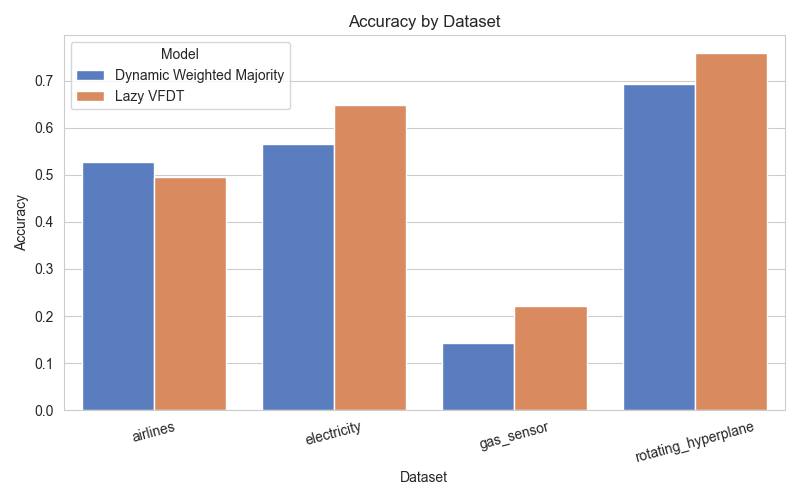
\includegraphics[width=0.8\linewidth]{tex/img/accuracy.png}
    \caption{Accuracy comparison across datasets.}
    \label{fig:accuracy}
\end{figure}

\begin{figure}[!h]
    \centering
    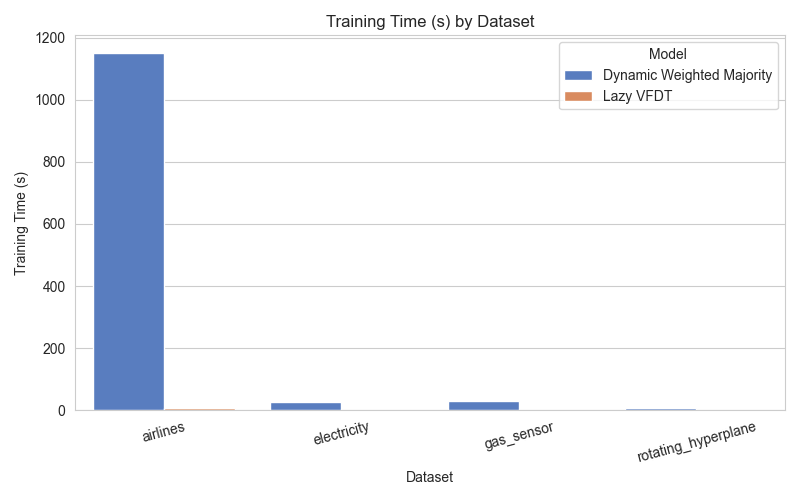
\includegraphics[width=0.8\linewidth]{tex/img/training_time.png}
    \caption{Training time comparison (log-scale recommended when presenting).}
    \label{fig:training-time}
\end{figure}

\begin{figure}[!h]
    \centering
    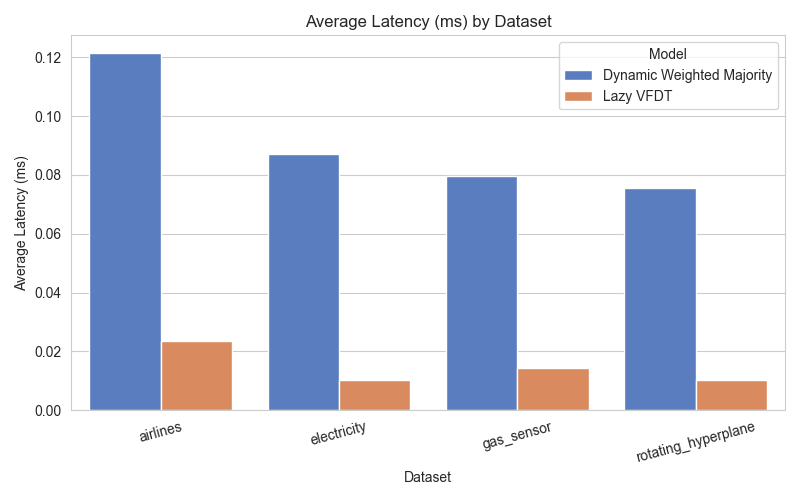
\includegraphics[width=0.8\linewidth]{tex/img/avg_latency.png}
    \caption{Average prediction latency comparison.}
    \label{fig:avg-latency}
\end{figure}

The figures emphasise Lazy VFDT’s consistent efficiency gains, even when DWM occasionally edges accuracy (e.g., Airlines).


\cleardoublepage
\chapter{Discussion}
\label{chap:discussion}

This chapter synthesises the empirical findings, focusing on the trade-offs between accuracy and efficiency, the impact of preprocessing/tuning, and the practical implications for deploying Lazy VFDT in streaming environments.

\section{Accuracy vs. Efficiency Trade-offs}
A clear pattern emerges: Lazy VFDT often matches or exceeds DWM accuracy on gradual or moderately noisy streams (Rotating Hyperplane, Electricity), while delivering 1--2 orders of magnitude faster training and significantly lower latency. On more complex multi-class streams (Gas Sensor, Airlines), DWM's ensembles can edge out accuracy, but the computational overhead is substantial. Practitioners must balance the marginal accuracy gains from ensembles against runtime constraints---especially when operating under tight latency budgets or limited compute resources. Lazy VFDT's single-tree architecture is attractive in such scenarios, provided modest tuning is applied.

\section{Impact of Preprocessing and Tuning}
Preprocessing choices strongly influence outcomes on multi-class, drifting sensors. Per-batch standardisation was essential for Gas Sensor data: without it, both methods performed poorly, but Lazy VFDT suffered more. Deeper trees (higher \texttt{max\_depth}, larger \texttt{grace\_period}) improved accuracy, albeit at the cost of larger node counts. These settings remain interpretable and easy to control, enabling practitioners to trade complexity for accuracy within predictable bounds. Airlines showed the limits of this tuning: even with scaling and deeper trees, Lazy VFDT remained a few points behind DWM, suggesting that additional features or hybrid strategies (e.g., small ensembles of Lazy VFDTs) might be beneficial.

\section{Practical Recommendations}
\begin{itemize}
    \item Use default Lazy VFDT settings (depth 6, grace 11, no scaling) for binary streams with gradual drift (e.g., Electricity) to get immediate efficiency gains.
    \item Apply dataset-aware presets: \texttt{--preset gas --scale-per-batch} for sensor drift, \texttt{--scale --ldt-max-depth 10 --ldt-grace-period 20} for Airlines-like streams.
    \item Consider ensembles only when accuracy gains justify the heavy training cost---for long-running streams, Lazy VFDT can be retrained or adapted far more frequently.
    \item Maintain logging (\texttt{results.csv}) and summary scripts to monitor when tuning drifts out of spec; adaptive parameter selection is a promising avenue for future work.
\end{itemize}

\section{Limitations}
This study focuses on a single baseline (DWM) and a select set of datasets. While representative, additional baselines (e.g., Adaptive Random Forests) and real-world streams (financial transactions, intrusion detection) would enrich the picture. The current evaluation also uses holdout + streamed test chunks rather than fully prequential evaluation; future work could integrate progressive validation and concept-drift detectors to stress-test Lazy VFDT under continuous deployment. Finally, the accuracy of both models on challenging multi-class streams remains modest---improving feature engineering, scaling strategies, or combining Lazy VFDT with lightweight ensembles could push performance further.

\cleardoublepage
\chapter{Conclusion}
\label{chap:conclusion}

This thesis introduced a practical evaluation of Lazy Very Fast Decision Trees (Lazy VFDT) for concept-drifting data streams. The main findings are:
\begin{itemize}
    \item Lazy VFDT matches or surpasses DWM accuracy on gradual-drift binary streams (Rotating Hyperplane, Electricity) while being one to two orders of magnitude more efficient in training and prediction latency.
    \item With dataset-specific preprocessing (per-batch scaling) and modest tuning (deeper trees), Lazy VFDT remains competitive on challenging multi-class sensor data, though absolute accuracy remains an open challenge.
    \item For large heterogeneous streams such as Airlines, Lazy VFDT trades a small accuracy penalty for dramatic reductions in computational cost, highlighting its suitability for resource-sensitive deployments.
\end{itemize}

Beyond accuracy metrics, the thesis contributes a reproducible experimentation framework, dataset conversion tools, aggregated results tables, and automated plots---all of which can be reused or extended for future studies.

\section{Future Work}
Several directions remain open:
\begin{itemize}
    \item \textbf{Adaptive parameter tuning}---automatically adjusting depth or grace period based on observed drift rather than relying on manual presets.
    \item \textbf{Additional baselines}---comparing Lazy VFDT with Adaptive Random Forests, Leveraging Bagging, or lightweight ensembles of Lazy VFDTs to broaden the empirical picture.
    \item \textbf{Prequential evaluation}---extending the current holdout-based protocol to fully prequential setups with drift detectors, enabling continuous deployment scenarios.
    \item \textbf{Hybrid models}---exploring combinations of lazy pruning with small ensembles to preserve accuracy on multi-class streams while retaining efficiency.
\end{itemize}

These enhancements would further clarify the circumstances under which Lazy VFDT is the preferred choice and how it can be integrated into production stream-processing pipelines.


 % Można też pisać rozdziały w jednym pliku.


%---------------
% Bibliografia
%---------------
\cleardoublepage % Zaczynamy od nieparzystej strony
\printbibliography
\clearpage

% Wykaz symboli i skrótów.
% Pamiętaj, żeby posortować symbole alfabetycznie
% we własnym zakresie. Makro \acronymlist
% generuje właściwy tytuł sekcji, w zależności od języka.
% Makro \acronym dodaje skrót/symbol do listy,
% zapewniając podstawowe formatowanie.

%--------------------------------------
% Spisy: rysunków, tabel, załączników
%--------------------------------------
\pagestyle{plain}

\listoffigurestoc    % Spis rysunków.
\vspace{1cm}         % vertical space
\listoftablestoc     % Spis tabel.
\vspace{1cm}         % vertical space
\listofappendicestoc % Spis załączników

%-------------
% Załączniki
%-------------

% Obrazki i tabele w załącznikach nie trafiają do spisów
\captionsetup[figure]{list=no}
\captionsetup[table]{list=no}

% Załącznik 1
\clearpage
\appendix{Nazwa załącznika 1}
\lipsum[1-3]
\begin{figure}[!h]
	\centering 
\includegraphics[width=0.5\linewidth]{logopw2.png}
	\caption{Obrazek w załączniku.}
\end{figure}
\lipsum[4-7]

% Załącznik 2
\clearpage
\appendix{Nazwa załącznika 2}
\lipsum[1-2]
\begin{table}[!h] \centering
    \caption{Tabela w załączniku.}
    \begin{tabular} {| c | c | r |} \hline
        Kolumna 1       & Kolumna 2 & Liczba \\ \hline\hline
        cell1           & cell2     & 60     \\ \hline
        \multicolumn{2}{|r|}{Suma:} & 123,45 \\ \hline
    \end{tabular}
\end{table}
\lipsum[3-4]

% Używając powyższych spisów jako szablonu,
% możesz dodać również swój własny wykaz,
% np. spis algorytmów.

\end{document} % Dobranoc.
